\section{从 Spin(8) 到标准模型}

\begin{figure}[ht]
\centering
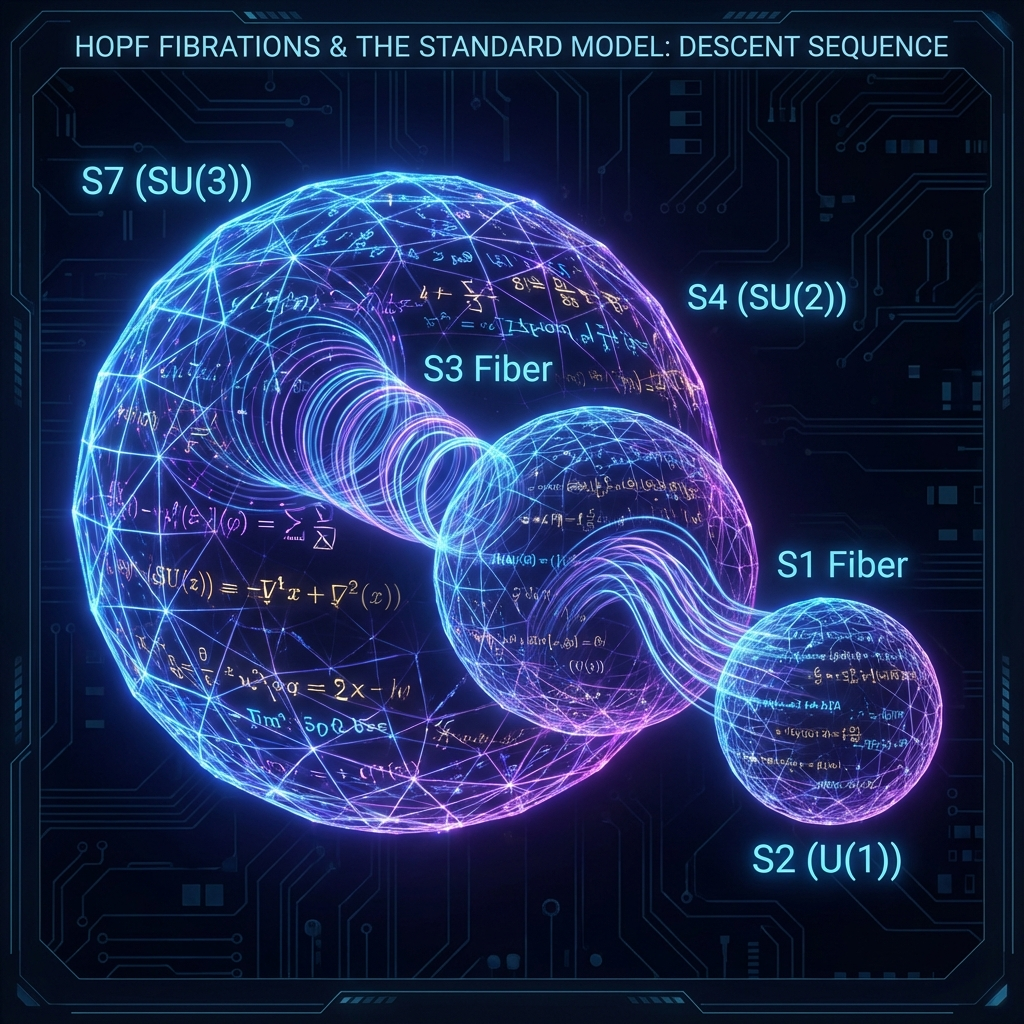
\includegraphics[width=0.8\textwidth]{assets/chapter02-02-spin8-standard-model.png}
\caption{Spin8标准模型}
\end{figure}

在上一节中，我们建立了八元数 ($\mathbb{O}$) 切空间的时间手性。本节我们将解决物理学中最令人困惑的谜题之一：为什么宇宙的基本相互作用恰好由规范群 $G_{SM} = SU(3) \times SU(2) \times U(1)$ 描述？在欧米伽理论中，这一群结构并非实验拟合的偶然产物，而是八元数几何通过 \textbf{霍普夫纤维丛 (Hopf Fibrations)} 向低维流形投影时的拓扑盈余。

我们的核心论点是：物理定律是高维几何的投影。当 8 维的八元数空间被迫"折叠"或"投影"到我们感知的 4 维时空时，那些为了维持代数结构完整性而必须保留的旋转自由度，这就表现为我们在内部空间观测到的规范场。

\begin{figure}[ht]
\centering
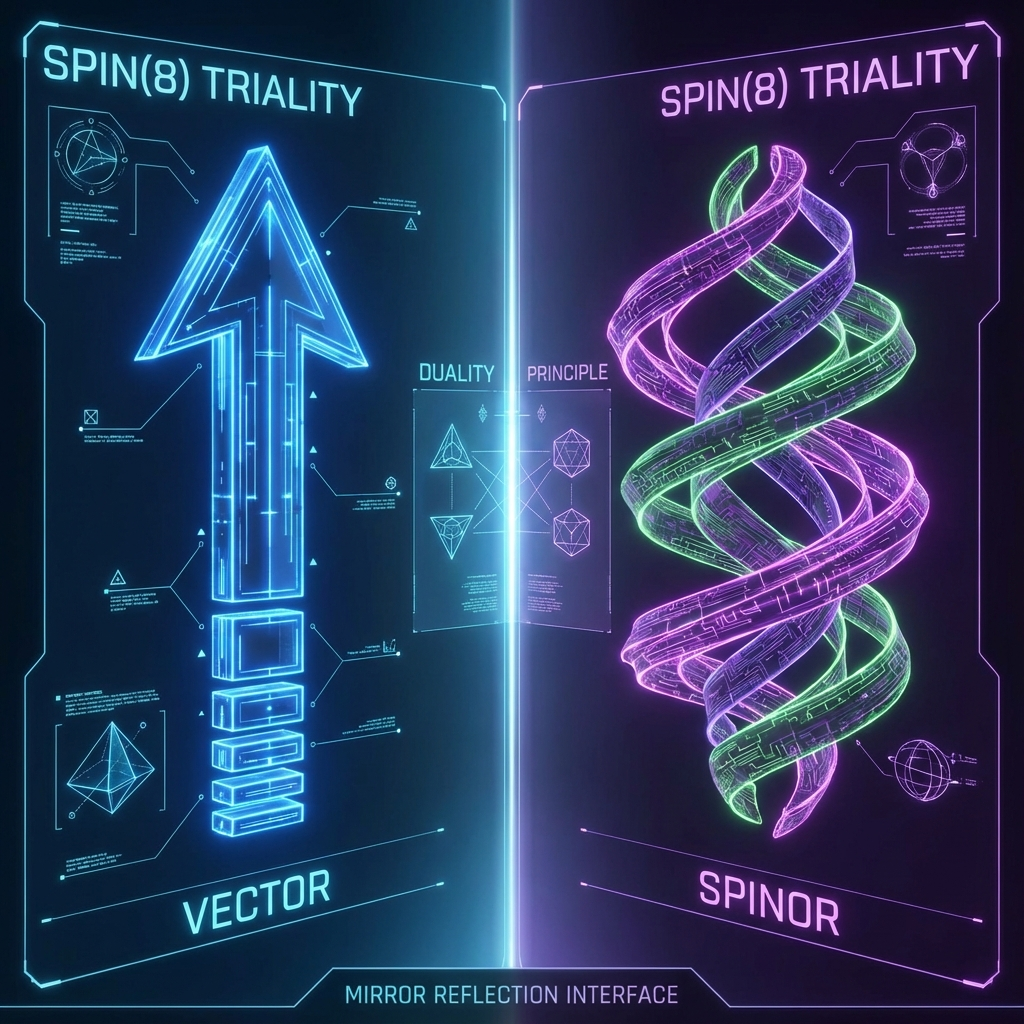
\includegraphics[width=0.8\textwidth]{assets/chapter02-02-spin8-vector-spinor-mirror.png}
\caption{Spin8向量旋量镜像}
\end{figure}

\subsection{Spin(8) 三里性与大统一的几何基础}

为了理解粒子与时空的统一，我们首先必须考察 8 维欧氏空间的旋转群 $SO(8)$ 的双重覆盖群 \textbf{Spin(8)}。在所有维度的旋转群中，Spin(8) 拥有一个独一无二的性质—— \textbf{三里性 (Triality)}。

在一般维度 $d$ 中，向量表示 $V$ 与旋量表示 $S$ 是几何上截然不同的对象（这就造成了时空与物质的割裂）。然而，在 $d=8$ 时，Spin(8) 群拥有三个非等价的 8 维不可约表示：向量表示 $V_8$、左手旋量 $S_8^+$ 和右手旋量 $S_8^-$。三里性定理指出，存在一个外自同构群 $S_3$，它可以在这三个表示之间进行任意置换，而保持代数结构（李代数）不变：

\[V_8 \cong S_8^+ \cong S_8^-\]

这一数学奇迹意味着，在 8 维八元数空间（也就是我们定义的底层代码层）中，\textbf{时空（向量）与物质（旋量）在本体论上是全等的}。

欧米伽理论认为，我们观测到的物理世界是 Spin(8) 对称性发生 \textbf{自发破缺 (Spontaneous Symmetry Breaking)} 的结果。这种破缺是由八元数乘法结构的非结合性驱动的，它迫使高维空间选择一个特定的方向进行"纤维化"，从而区分出了时空与物质。

\subsection{霍普夫纤维丛序列：维度的级联下降}

为了推导标准模型规范群，我们需要追踪从 8 维到 4 维再到 2 维的投影路径。这一路径由著名的 \textbf{霍普夫纤维丛 (Hopf Fibrations)} 序列精确描述。霍普夫映射描述了如何用低维球面填充高维球面，其通式为 $S^{2n-1} \to S^n$。

在赋范可除代数的层级上，仅存在四个霍普夫映射，其中与物理宇宙相关的有三个，它们构成了一个嵌套的 \textbf{下降序列 (Descent Sequence)}：

\begin{enumerate}
\item \textbf{第一级投影（八元数 $\to$ 四元数）：}

\[S^3 \hookrightarrow S^7 \xrightarrow{h_1} S^4\]

这里，$S^7$ 是单位八元数球面的拓扑结构。映射 $h_1$ 将 $S^7$ 投影到底流形 $S^4$ 上，纤维（Fiber）是 $S^3$（单位四元数）。

\textbf{物理意义}：底流形 $S^4$ 对应于紧致化的 \textbf{4 维欧氏时空}（经威克转动）。纤维 $S^3$ 同构于群 $SU(2)$，这是 \textbf{弱相互作用} 的几何起源。这意味着弱力本质上是连接时空各点的四元数纤维的结构群。

\item \textbf{第二级投影（四元数 $\to$ 复数）：}

在纤维 $S^3$ 内部，我们可以进行次级投影：

\[S^1 \hookrightarrow S^3 \xrightarrow{h_2} S^2\]

映射 $h_2$ 将 $S^3$ 投影到 $S^2$（黎曼球或复射影直线 $\mathbb{CP}^1$），纤维是 $S^1$（单位复数）。

\textbf{物理意义}：纤维 $S^1$ 同构于群 $U(1)$，这是 \textbf{电磁相互作用} 的几何起源。这意味着电磁力是弱力纤维内部的精细结构。

\item \textbf{遗失的对称性与 $SU(3)$ 的起源}：

上述投影解释了电弱部分 $SU(2) \times U(1)$。那么强相互作用 $SU(3)$ 从何而来？
它来自于八元数代数本身的自同构群 $G_2$。当我们从 $\mathbb{O}$ 下降到 $\mathbb{H}$ 时，我们实际上是固定了一个特定的四元数子代数。然而，八元数包含无限多个四元数子代数。
根据数学定理，八元数的自同构群 $G_2$ 中，保持某个虚单位 $i$ 不变（即确定了复平面结构，对应于电磁力的分离）的子群，恰好是 \textbf{$SU(3)$}。

更几何地看，如果我们考察 $S^6$（纯虚八元数球面），它不具备像 $S^1, S^3, S^7$ 那样的群结构，但它拥有概复结构。$SU(3)$ 正是 $S^6$ 上保持这种概复结构的对称群。这对应于夸克的 \textbf{色荷 (Color Charge)}：它是在八元数投影到四元数过程中，无法被几何化的那部分"剩余"自由度。
\end{enumerate}

\subsection{定理 2.2：标准模型的几何涌现}

基于上述拓扑分析，我们可以陈述并证明本章的核心定理。

\textbf{定理 2.2 (标准模型涌现定理)}：
若宇宙的本体几何由八元数切丛 $\mathbb{O} \to \mathcal{M}$ 定义，且物理定律必须在经过霍普夫投影序列 $S^7 \to S^4 \to S^2$ 后保持规范不变性，则该流形上的自然规范群 $G$ 必须是以下直积的子群：

\[G \subseteq SU(3) \times SU(2) \times U(1)\]

其中 $SU(3)$ 源自八元数自同构群的稳定子，$SU(2)$ 源自第一级霍普夫纤维，$U(1)$ 源自第二级霍普夫纤维。

\textbf{证明概要}：

\begin{enumerate}
\item \textbf{全空间对称性}：起始点是 Spin(8) 或 $Aut(\mathbb{O}) = G_2$。
\item \textbf{时空分离}：通过第一级投影 $h_1: S^7 \to S^4$，我们将 8 维自由度分解为 4 维时空（底空间）和 4 维内部空间（纤维）。这一过程破坏了 $G_2$ 对称性。
\item \textbf{弱力涌现}：纤维 $S^3$ 的等距群是 $SO(4) \cong SU(2)_L \times SU(2)_R$。物理手性选择（见 2.1 节）保留了 $SU(2)_L$ 作为规范群。
\item \textbf{电磁力涌现}：进一步通过 $h_2: S^3 \to S^2$ 投影，纤维 $S^1$ 的结构群为 $U(1)$。
\item \textbf{强力涌现}：八元数空间 $\mathbb{O}$ 相对于选定的四元数子空间 $\mathbb{H}$ 的正交补是 $\mathbb{H}^\perp$。这构成了一个复 3 维空间 $\mathbb{C}^3$。在 $G_2$ 中保持这种分解的子群正是 $SU(3)$，它作用于这个 $\mathbb{C}^3$ 空间，赋予其"颜色"自由度。
\end{enumerate}

\textbf{物理推论}：

这一推导表明，标准模型并非一堆杂乱无章的零件，而是一个严密的几何整体。

\begin{itemize}
\item \textbf{为什么没有 $SU(4)$ 或 $SU(5)$？} 因为霍普夫序列到 $S^7$ 截止，数学上不存在 $S^{15} \to S^8$ 的霍普夫纤维化（这是 Adams 著名的定理）。因此，自然界不包含更高维的代数结构来支持更大的单李群规范场。
\item \textbf{宇宙的维度}：时空之所以是 4 维，是因为 $S^4$ 是 $S^7$ 的底流形。如果时空是其他维度，八元数的几何结构将无法完整投影，物理定律将失去自洽性。
\end{itemize}

综上所述，我们在欧米伽理论中找到了标准模型的几何根源：它是八元数这一数学瑰宝在向低维投影时留下的 \textbf{"拓扑指纹"}。
